\subsection{Diagramma UML delle classi}
In questa sezione sono stati riportati due diagrammi delle classi: il primo, in Figura \ref{fig:Class Diagram - v3}, rappresenta il diagramma delle classi dotato di tutte le dipendenze tra le classi, mentre il secondo, in Figura \ref{fig:Simplified Class Diagram - v3}, rappresenta il diagramma delle classi privato di alcune dipendenze esclusivamente al fine di renderne la comprensione più agevole.

Si tenga inoltre conto del fatto che le classi:
\begin{itemize}
    \item \texttt{CampoNativo}
    \item \texttt{Categoria}
    \item \texttt{Configuratore}
    \item \texttt{Fruitore}
    \item \texttt{Gerarchia}
    \item \texttt{Giorno}
    \item \texttt{InfoScambio}
    \item \texttt{IntervalloOrario}
    \item \texttt{Offerta}
    \item \texttt{Orario}
    \item \texttt{User}
    \item \texttt{UserDataStore}
\end{itemize}
implementano l'interfaccia \texttt{Serializable}, nonostante tale relazione non sia esplicitamente riportata nei diagrammi delle classi al fine di semplificare il layout dei diagrammi stessi.

\begin{figure}[!]
    \centering
    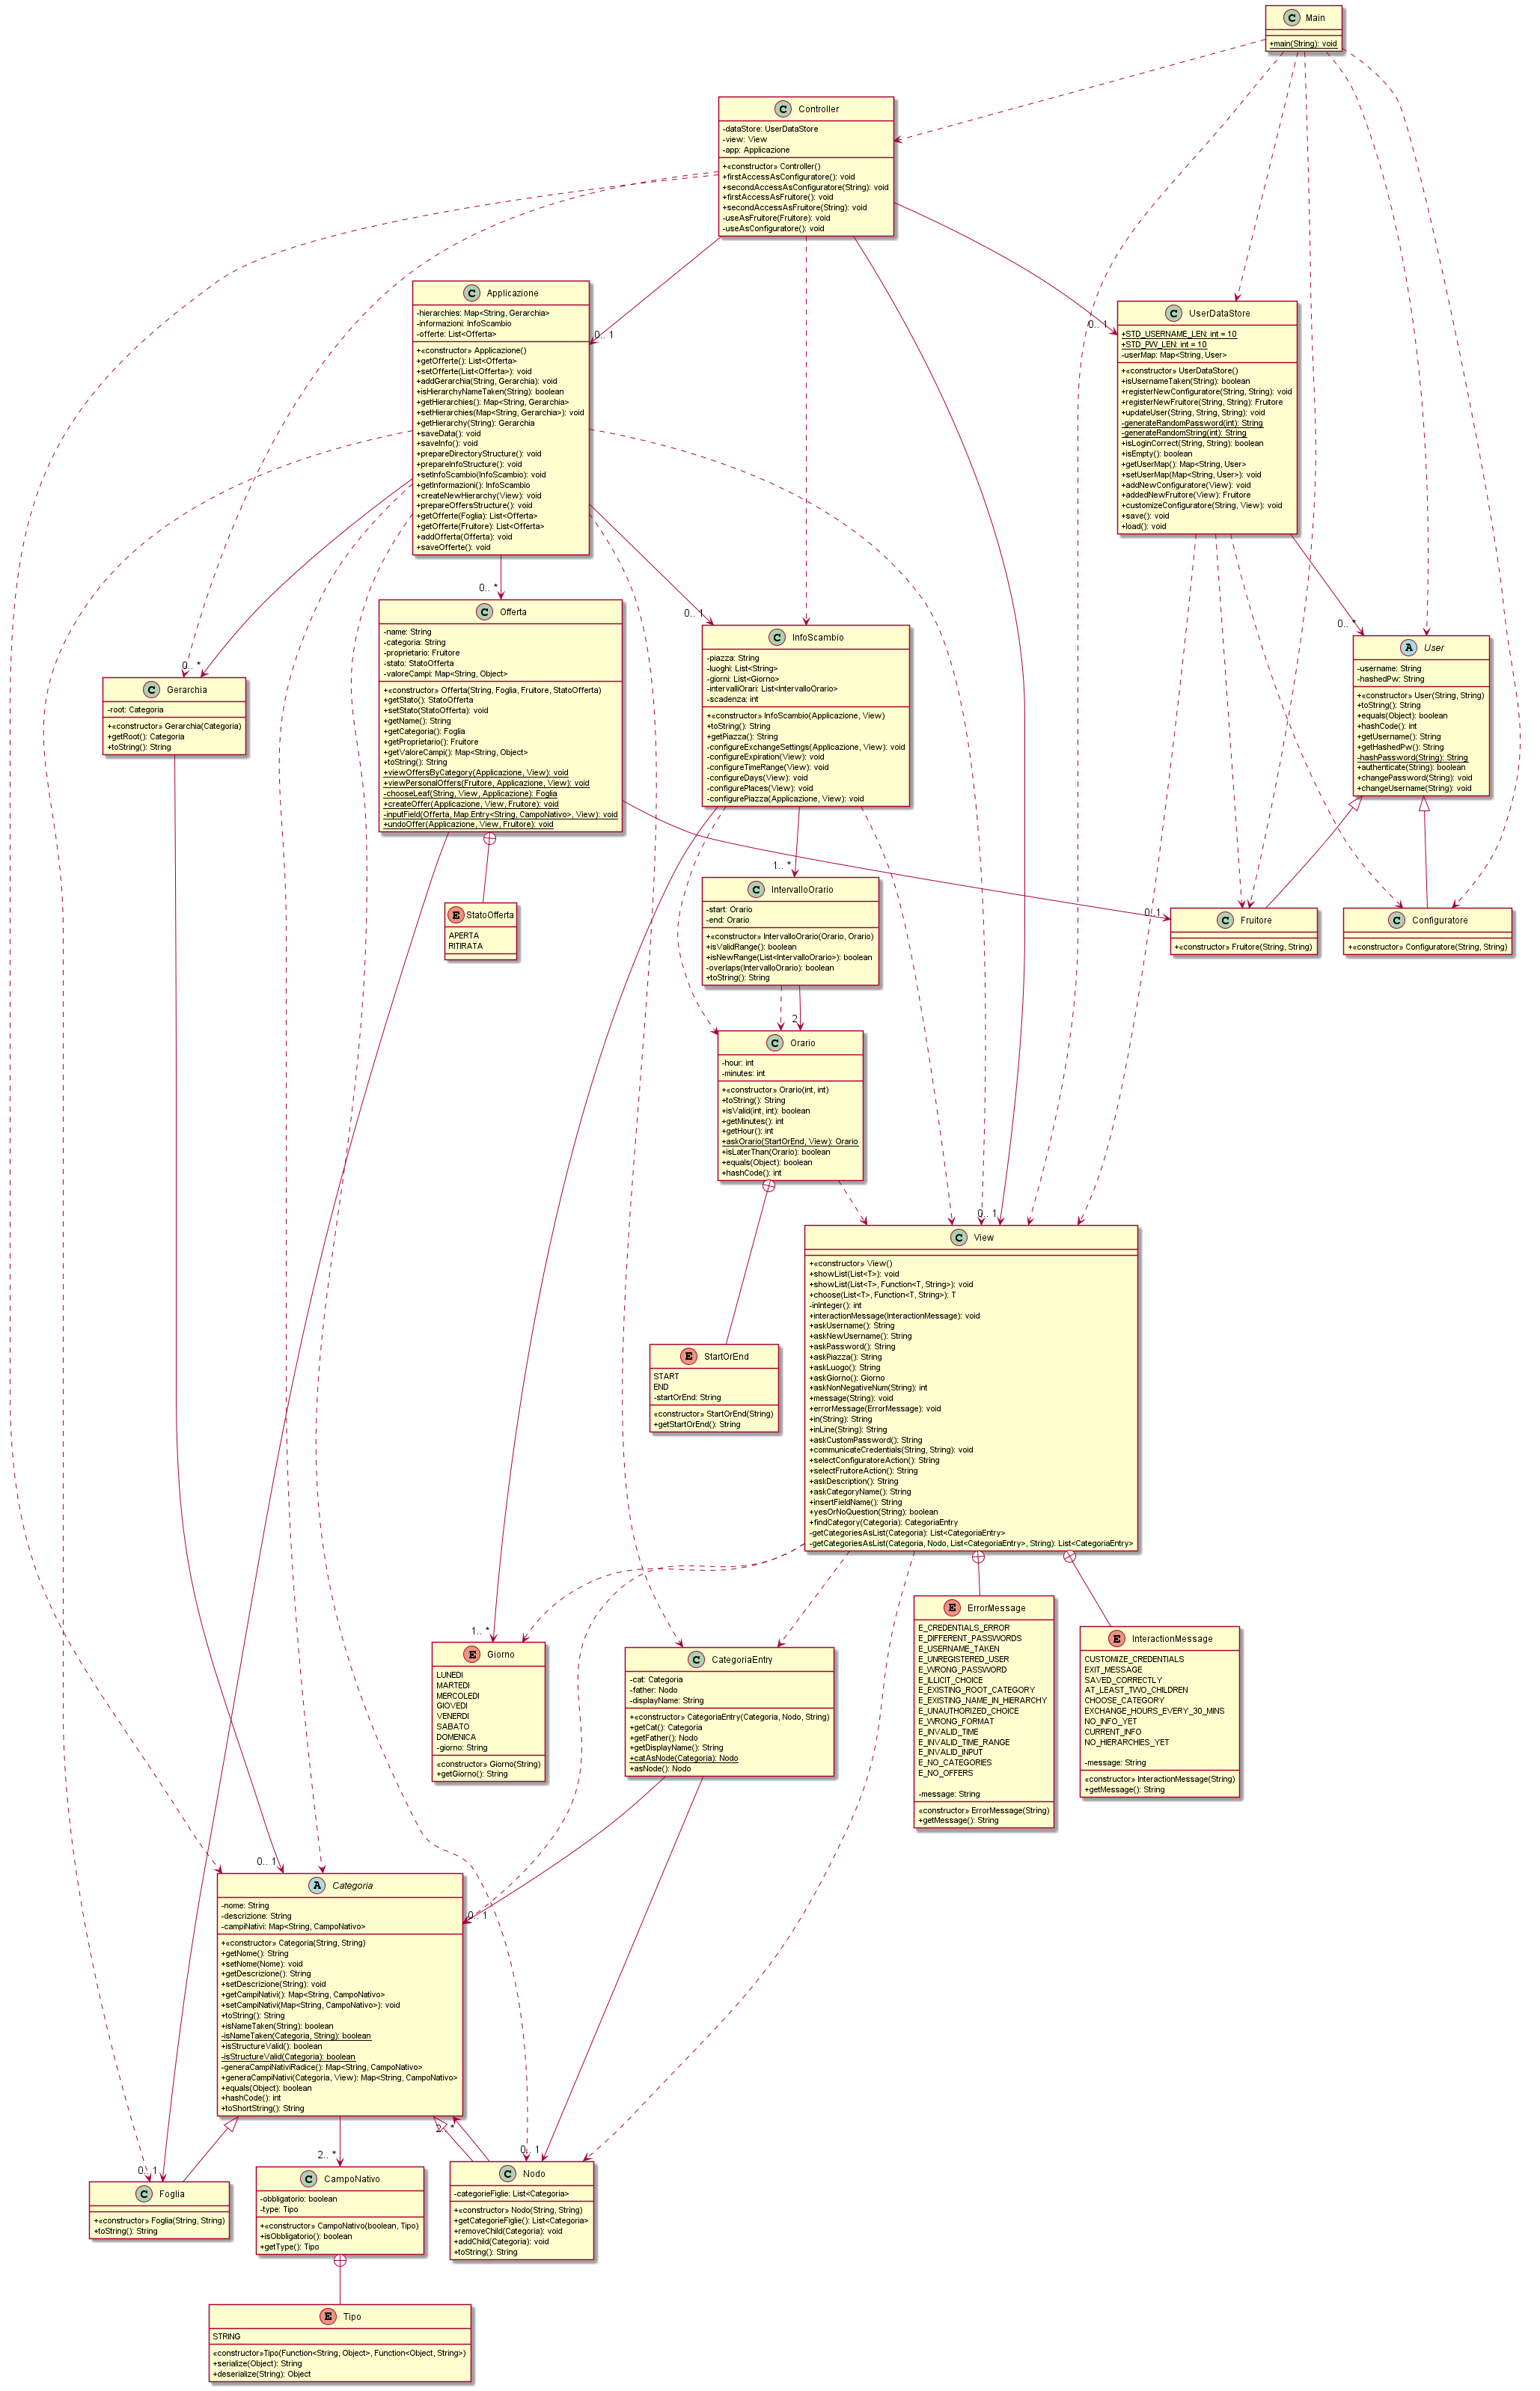
\includegraphics[width=16cm]{imagesV3/Class diagram-version3.png}
    \caption{\label{fig:Class Diagram - v3}Diagramma UML delle classi - Versione 3}
\end{figure} 

La classe \texttt{View} contiene i metodi (non indicati per esteso nel diagramma delle classi realizzato prima dell'effettiva stesura del codice) necessari per interagire e comunicare con l'utente, ricevendo i dati da lui inseriti oppure comunicando messaggi da parte del sistema.

La classe \texttt{UserDataStore} contiene i metodi necessari per la gestione dei dati relativi agli utenti che dovranno poi essere salvati in modo persistente. La classe ha il compito di gestire la registrazione di un nuovo utente, l'aggiornamento delle credenziali (se si tratta di un profilo Configuratore) e la verifica della correttezza delle informazioni introdotte in fase di login, oltre al salvataggio e al caricamento dei dati. 

La classe \texttt{User} è una classe astratta estesa dalla classe \texttt{Configuratore} e dalla classe \texttt{Fruitore}: ogni utente sarà dotato di username e password. La password, in particolare, viene salvata direttamente dopo aver effettuato l'hashing, in modo da garantire un livello di sicurezza basilare relativamente alle informazioni private degli utenti. La classe \texttt{User} è dotata di metodi per l'autenticazione dell'utente e per la modifica delle credenziali.

La classe \texttt{Applicazione} permette di tenere traccia delle gerarchie contenute nell'applicazione, delle informazioni di scambio e delle offerte inserite dagli utenti. 
Essa contiene infatti un metodo che verifica se il nome di una categoria radice di una gerarchia è già utilizzato dalla categoria radice di un'altra gerarchia, un metodo che permette di creare e aggiungere una nuova gerarchia, metodi che permettono di ottenere le gerarchie presenti nell'applicazione o di assegnare loro i valori desiderati, metodi che permettono di salvare i dati contenuti nelle gerarchie e di caricare i dati salvati durante gli utilizzi precedenti dell'applicazione.
Inoltre contiene i metodi necessari a leggere da file e salvare su file le informazioni di scambio e le offerte contenute nell'applicazione. 

La classe \texttt{Gerarchia} permette di tenere traccia del contenuto di ogni gerarchia: ogni gerarchia è caratterizzata da una categoria radice che, a seconda che sia istanza della classe \texttt{Foglia} o \texttt{Nodo}, può avere o meno delle sottocategorie (a loro volta istanze della classe \texttt{Foglia} o \texttt{Nodo}). 

La classe \texttt{Categoria} è una classe astratta che è estesa dalla classe \texttt{Foglia} e dalla classe \texttt{Nodo}. Ogni categoria è dotata di nome obbligatorio, descrizione facoltativa e un insieme di campi nativi (due dei quali presenti di default per la categoria radice di una gerarchia) ereditati poi da ogni categoria figlia di un nodo.
La classe \texttt{Nodo}, in particolare, è dotata di una lista di categorie figlie che possono a loro volta essere foglie o nodi. Per questo motivo la classe \texttt{Nodo} è dotata di metodi che permettono di aggiungere o rimuovere una categoria figlia e di un metodo che permette di ottenere tutte le categorie figlie.

La classe \texttt{CampoNativo} tiene traccia dell'obbligatorietà della compilazione di un campo, nativo o ereditato, relativo a una categoria e del tipo del campo (di default si tratta di stringhe). 

La classe \texttt{CategoriaEntry} tiene traccia dell'associazione tra una categoria e la sua categoria padre; essa contiene pertanto i metodi necessari a recuperare le informazioni relative a tale relazione (percorso dalla categoria radice alla categoria corrente, categoria padre e categoria corrente) e dei metodi per trasformare una categoria da Foglia a Nodo e associarla alla propria categoria padre.

La classe \texttt{Controller} contiene metodi per consentire l'accesso a un profilo Configuratore, differenziando tra il caso di registrazione e quello di accesso standard. Ognuno di questi metodi richiama poi uno o più ulteriori metodi che permettono l'utilizzo delle funzionalità a cui l'utente è autorizzato ad accedere; contiene inoltre metodi per consentire l'accesso a un profilo Fruitore, differenziando, come nel caso del configuratore, tra il caso di registrazione e quello di accesso, richiamando uno o più metodi che consentono di utilizzare tutte le funzionalità a cui l'utente è autorizzato ad accedere.

La classe \texttt{Main} contiene il solo metodo main che permette di interagire con l'applicazione selezionando l'azione da compiere tra accesso, registrazione o uscita dall'applicazione.

La classe \texttt{InfoScambio} gestisce le informazioni di scambio che devono essere impostate dall'utente Configuratore.

La classe \texttt{IntervalloOrario} contiene metodi per validare la correttezza di un intervallo orario introdotto dall'utente, assicurandosi che l'intervallo non sia ancora stato inserito tra le informazioni di scambio e che non si sovrapponga ad altri intervalli già presenti.

La classe \texttt{Orario} contiene metodi per validare la correttezza di un singolo orario introdotto dall'utente, assicurando che esso sia nel formato \textit{[hh:mm]} e che i minuti possano essere o 00 oppure 30, in quanto gli scambi possono avvenire solo allo scoccare dell'ora o della mezz'ora.

La classe \texttt{Offerta} contiene metodi per la gestione delle offerte; in particolare ne consente la creazione da parte dell'utente selezionando la categoria foglia di appartenenza, impostando un nome e il valore dei campi nativi (obbligatori e facoltativi); permette inoltre di gestire lo stato delle offerte e visualizzare informazioni sulle offerte presenti nell'applicazione.

\begin{figure}[!]
    \centering
    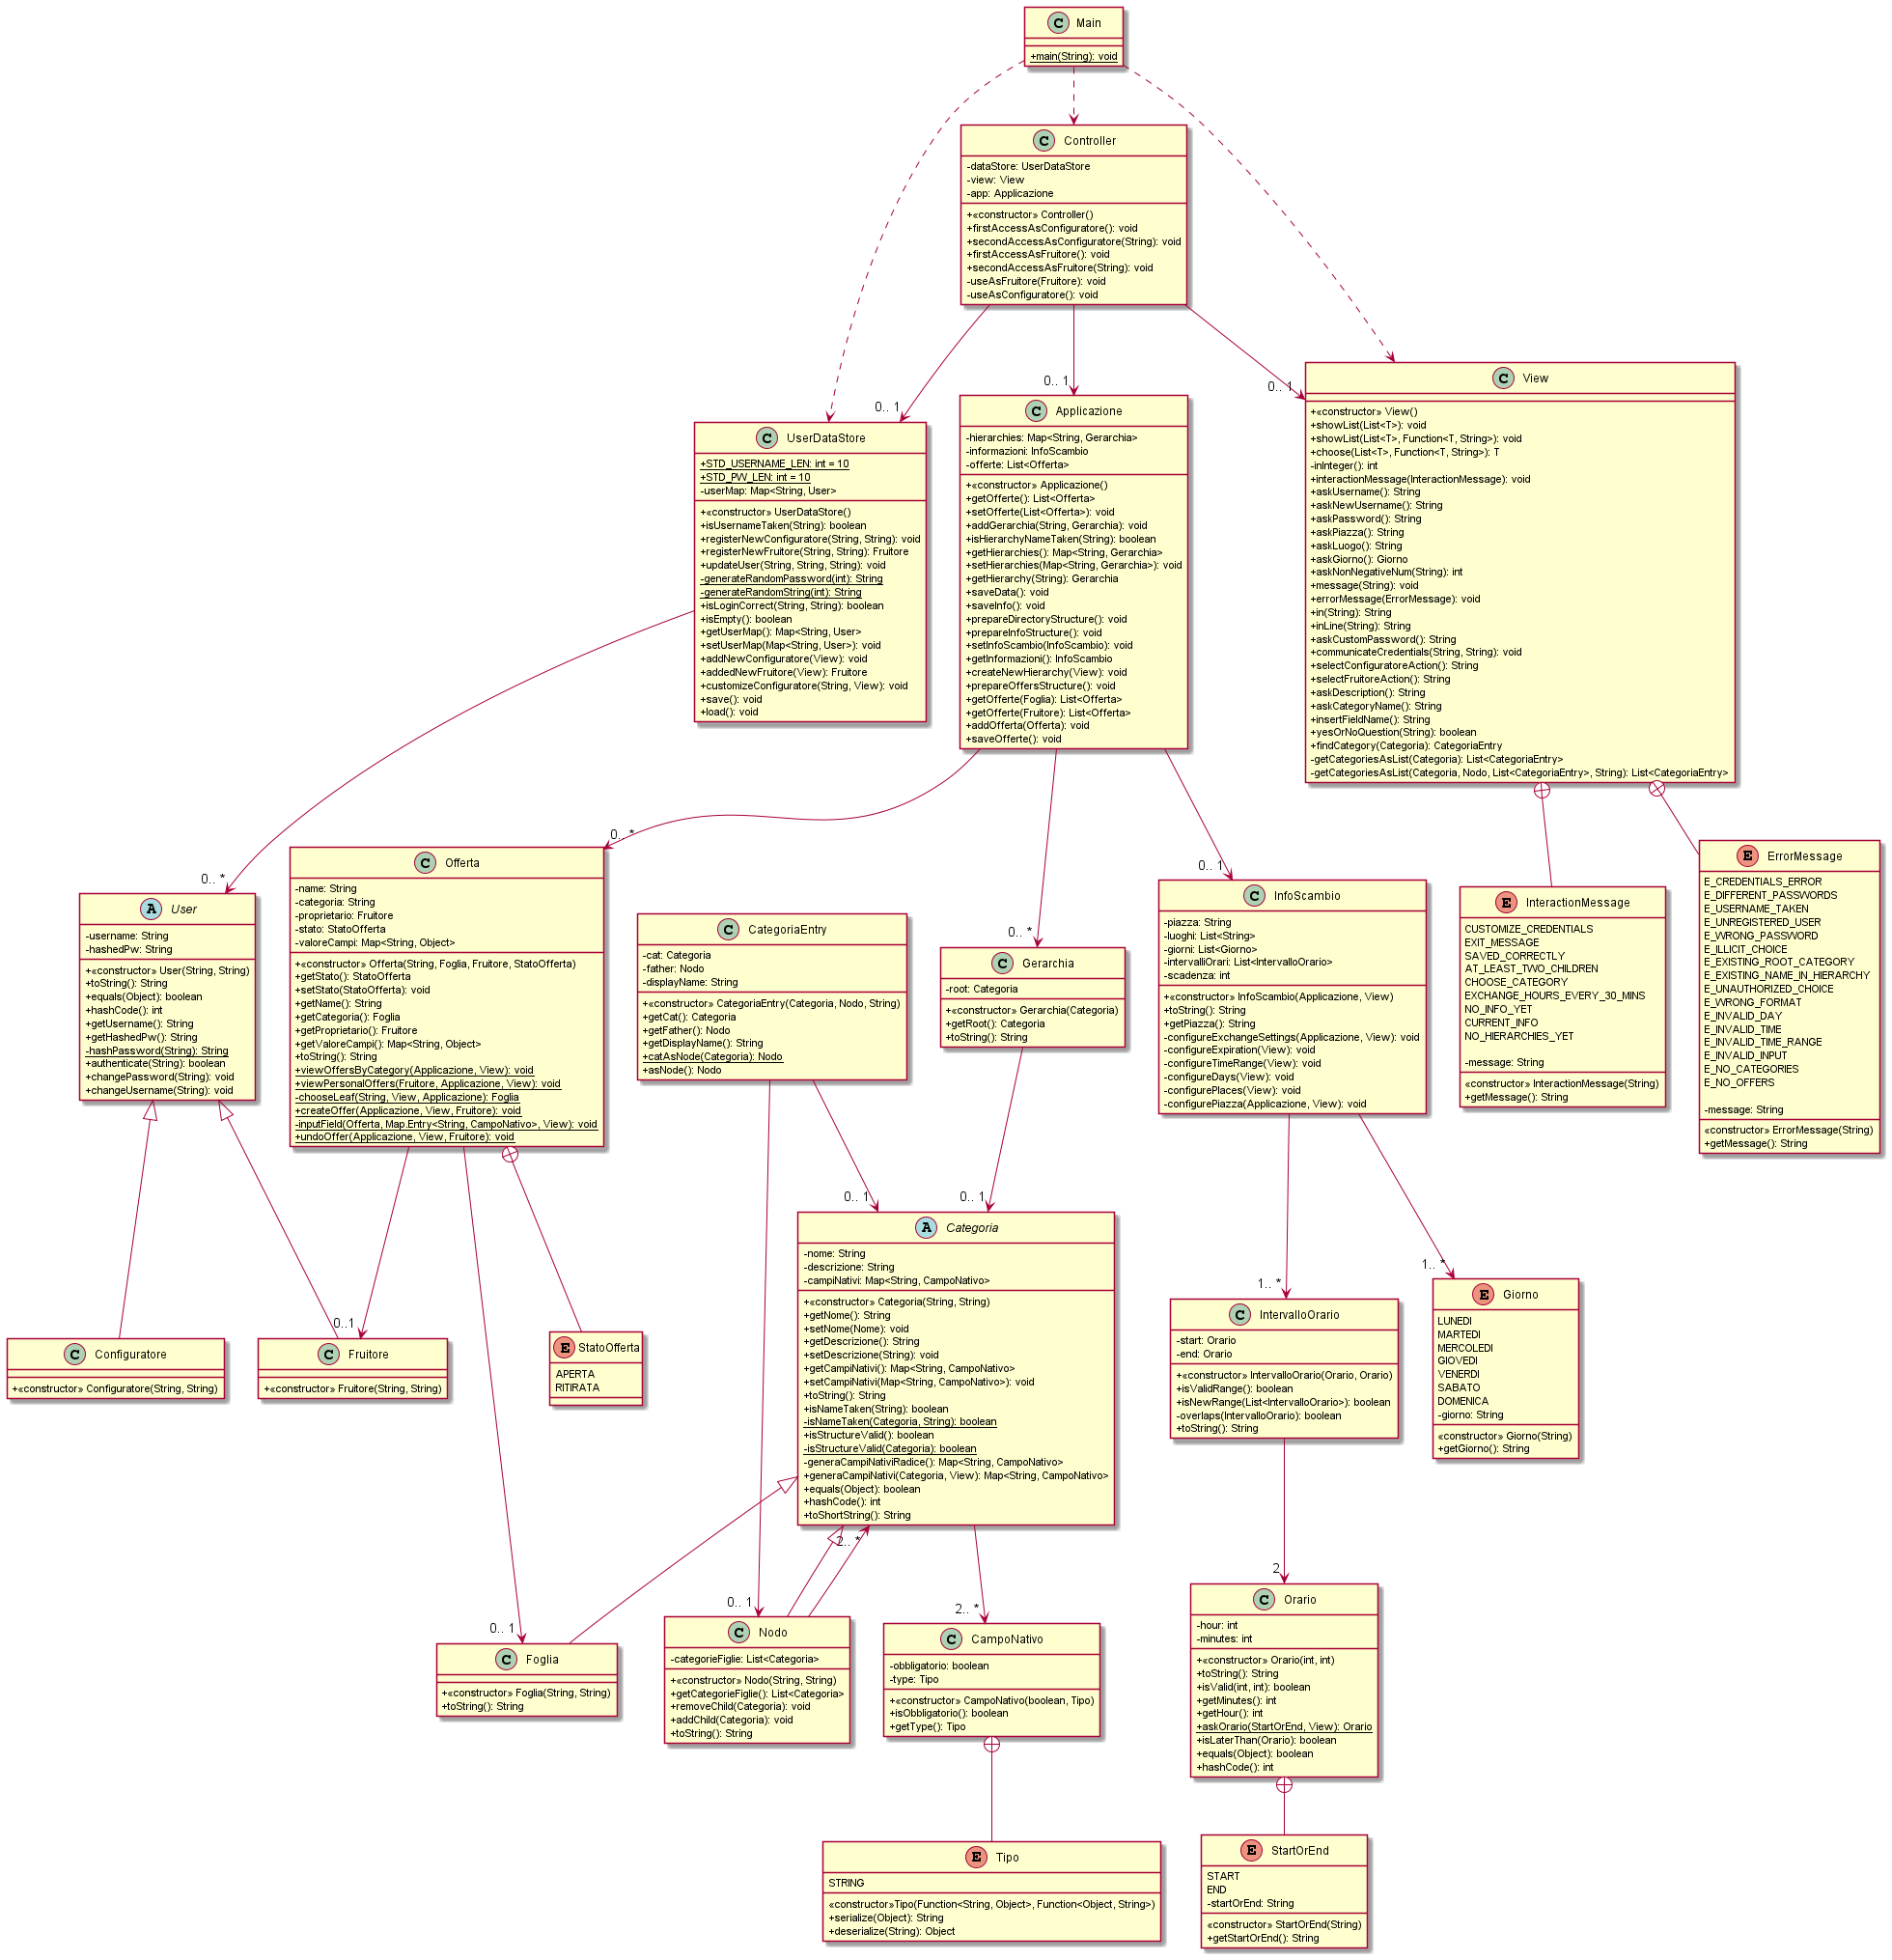
\includegraphics[width=16cm]{imagesV3/partial class diagram.png}
    \caption{\label{fig:Simplified Class Diagram - v3}Diagramma UML delle classi semplificato - Versione 3}
\end{figure}
\bigskip